The \verb=Analysis= module reads the ADC signal and puts out information on how to draw two bars (one for each speaker) that reflect the amplitude of said signal. Since we want bars for before and after modulation, we'll use two instances of the same module. 

The required inputs include a left or right selection signal to specify which stereo channel we are about to analyse, two 16 bit signed ADC/DAC signals (left and right), and \verb=vsync= lined from \verb+VGA_Driver+. There are two 8-bit unsigned output signals (once again, one left, one right). They determine the height of the bar which the \verb=VGA_Driver= should render.

The incoming signals are low pass filtered with a saturation time of approximately 100 ms (4096 sample cycles) as seen in figure \ref{fig:lowpass}, resulting in a measurement of the signal's amplitude. A signal proportional to the logarithm of the value is then passed on as \verb+bar+ to \verb+VGA_Driver+ synced by \verb+vsync+.

\begin{figure}[h]
\centering
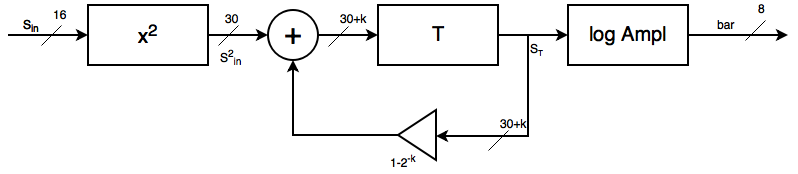
\includegraphics[width=16cm]{lowpass}
\caption{The low pass filter. $k$ is chosen by the approximation $\frac{1}{10}\mathrm{\ s} = 2^k\cdot\frac{1}{48800}\Rightarrow 2^k=4880\approx 2^{12}\Rightarrow k = 12 $}
\label{fig:lowpass}
\end{figure}


\verb=lrsel= determines which stereo channel should be read and thus which bar height should be written to at any given time.


